\documentclass[12pt,a4paper]{report}

% Essential packages
\usepackage[utf8]{inputenc}
\usepackage[T1]{fontenc}
\usepackage{times}
\usepackage[margin=1in]{geometry}
\usepackage{fancyhdr}
\usepackage{titlesec}
\usepackage{tocloft}
\usepackage{amsmath,amsfonts,amssymb}
\usepackage{graphicx}
\usepackage{booktabs}
\usepackage{longtable}
\usepackage{array}
\usepackage{listings}
\usepackage{xcolor}
\usepackage{hyperref}
\usepackage{cite}
\usepackage{setspace}
\usepackage{caption}
\usepackage{subcaption}

% Configure listings
\lstset{
    basicstyle=\ttfamily\footnotesize,
    breaklines=true,
    frame=single,
    numbers=left,
    numberstyle=\tiny,
    tabsize=2,
    showstringspaces=false
}

% Configure hyperref
\hypersetup{
    colorlinks=true,
    linkcolor=black,
    citecolor=blue,
    urlcolor=blue,
    pdftitle={3D Point Cloud Semantic Segmentation},
    pdfauthor={Arnav Kapoor}
}

% Page setup
\pagestyle{fancy}
\fancyhf{}
\fancyhead[L]{\leftmark}
\fancyhead[R]{\thepage}
\renewcommand{\headrulewidth}{0.4pt}

% Title formatting
\titleformat{\chapter}[display]
{\normalfont\Large\bfseries}{\chaptertitlename\ \thechapter}{20pt}{\Huge}
\titlespacing*{\chapter}{0pt}{-30pt}{40pt}

% Spacing
\onehalfspacing

% Document metadata
\title{3D Point Cloud Semantic Segmentation using Deep Learning}
\author{Arnav Kapoor}
\date{Summer 2025}

\begin{document}

% Title Page
\begin{titlepage}
    \centering
    \vspace*{1cm}
    
    {\LARGE\textbf{3D Point Cloud Semantic Segmentation using Deep Learning}}
    
    \vspace{0.5cm}
    {\Large An Internship Report}
    
    \vspace{2cm}
    
    {\large Submitted by}\\
    \vspace{0.5cm}
    {\Large\textbf{Arnav Kapoor}}
    
    \vspace{2cm}
    
    
\includegraphics[width=3cm]{logo.png}
    
    \vspace{1cm}
    
    {\large Under the supervision of}\\
    \vspace{0.5cm}
    {\Large\textbf{Prof. Vaibhav Kumar}}
    
    \vspace{2cm}
    
    {\large GeoAI4Cities Research Group}\\
    {\large Summer 2025}
    
\end{titlepage}

% Table of Contents
\pagenumbering{roman}
\tableofcontents
\newpage

% List of Figures - Simplified
\listoffigures
\addcontentsline{toc}{chapter}{List of Figures}
\newpage

% List of Tables
\listoftables
\addcontentsline{toc}{chapter}{List of Tables}
\newpage

% Main Content
\pagenumbering{arabic}

\chapter{Introduction}

Point cloud semantic segmentation is a fundamental task in computer vision and robotics, enabling machines to understand and interpret 3D environments. This internship at GeoAI4Cities focused on developing efficient deep learning solutions for real-time point cloud processing on edge computing platforms.

\section{Background}

Recent advances in 3D sensing technologies and deep learning have enabled sophisticated point cloud analysis. However, deploying these models on resource-constrained edge devices remains challenging due to computational and memory limitations.

\section{Objectives}

\begin{itemize}
    \item Implement and evaluate state-of-the-art point cloud segmentation models
    \item Optimize models for edge computing platforms (NVIDIA Jetson series)
    \item Integrate ZED camera for real-time point cloud acquisition
    \item Achieve real-time performance while maintaining accuracy
\end{itemize}

\section{Significance}

This work contributes to democratizing 3D vision capabilities on affordable hardware, enabling applications in autonomous vehicles, robotics, and augmented reality.

\chapter{Literature Review}

\section{Point Cloud Deep Learning}

\textbf{PointNet} \cite{qi2017pointnet} introduced the first deep learning approach for direct point cloud processing, using symmetric functions to handle unordered point sets.

\textbf{PointNet++} \cite{qi2017pointnetplus} enhanced PointNet with hierarchical feature learning, improving local structure understanding.

\textbf{PVCNN} \cite{liu2019point} combined point-based and voxel-based approaches for efficient processing.

\textbf{RandLA-Net} \cite{hu2020randla} addressed scalability through random sampling and local feature aggregation.

\textbf{SONATA} \cite{facebook2023sonata} provided a unified framework for multiple point cloud tasks.

\section{Edge Computing for 3D Vision}

Edge deployment requires careful balance between accuracy and efficiency. Key challenges include memory constraints, computational limitations, and power consumption.

\section{Datasets and Benchmarks}

\begin{itemize}
    \item \textbf{ShapeNet} \cite{chang2015shapenet}: Large-scale 3D shape dataset
    \item \textbf{S3DIS} \cite{armeni2016s3dis}: Indoor scene understanding
    \item \textbf{SemanticKITTI} \cite{behley2019semantickitti}: Autonomous driving scenarios
\end{itemize}

\chapter{Methodology}

\section{Development Environment}

The development environment consisted of:
\begin{itemize}
    \item NVIDIA RTX 3070 for training
    \item NVIDIA Jetson Xavier NX for edge deployment
    \item ZED 2i camera for data acquisition
    \item Ubuntu 20.04 with CUDA 11.8
\end{itemize}

\begin{figure}[htbp]
    \centering
    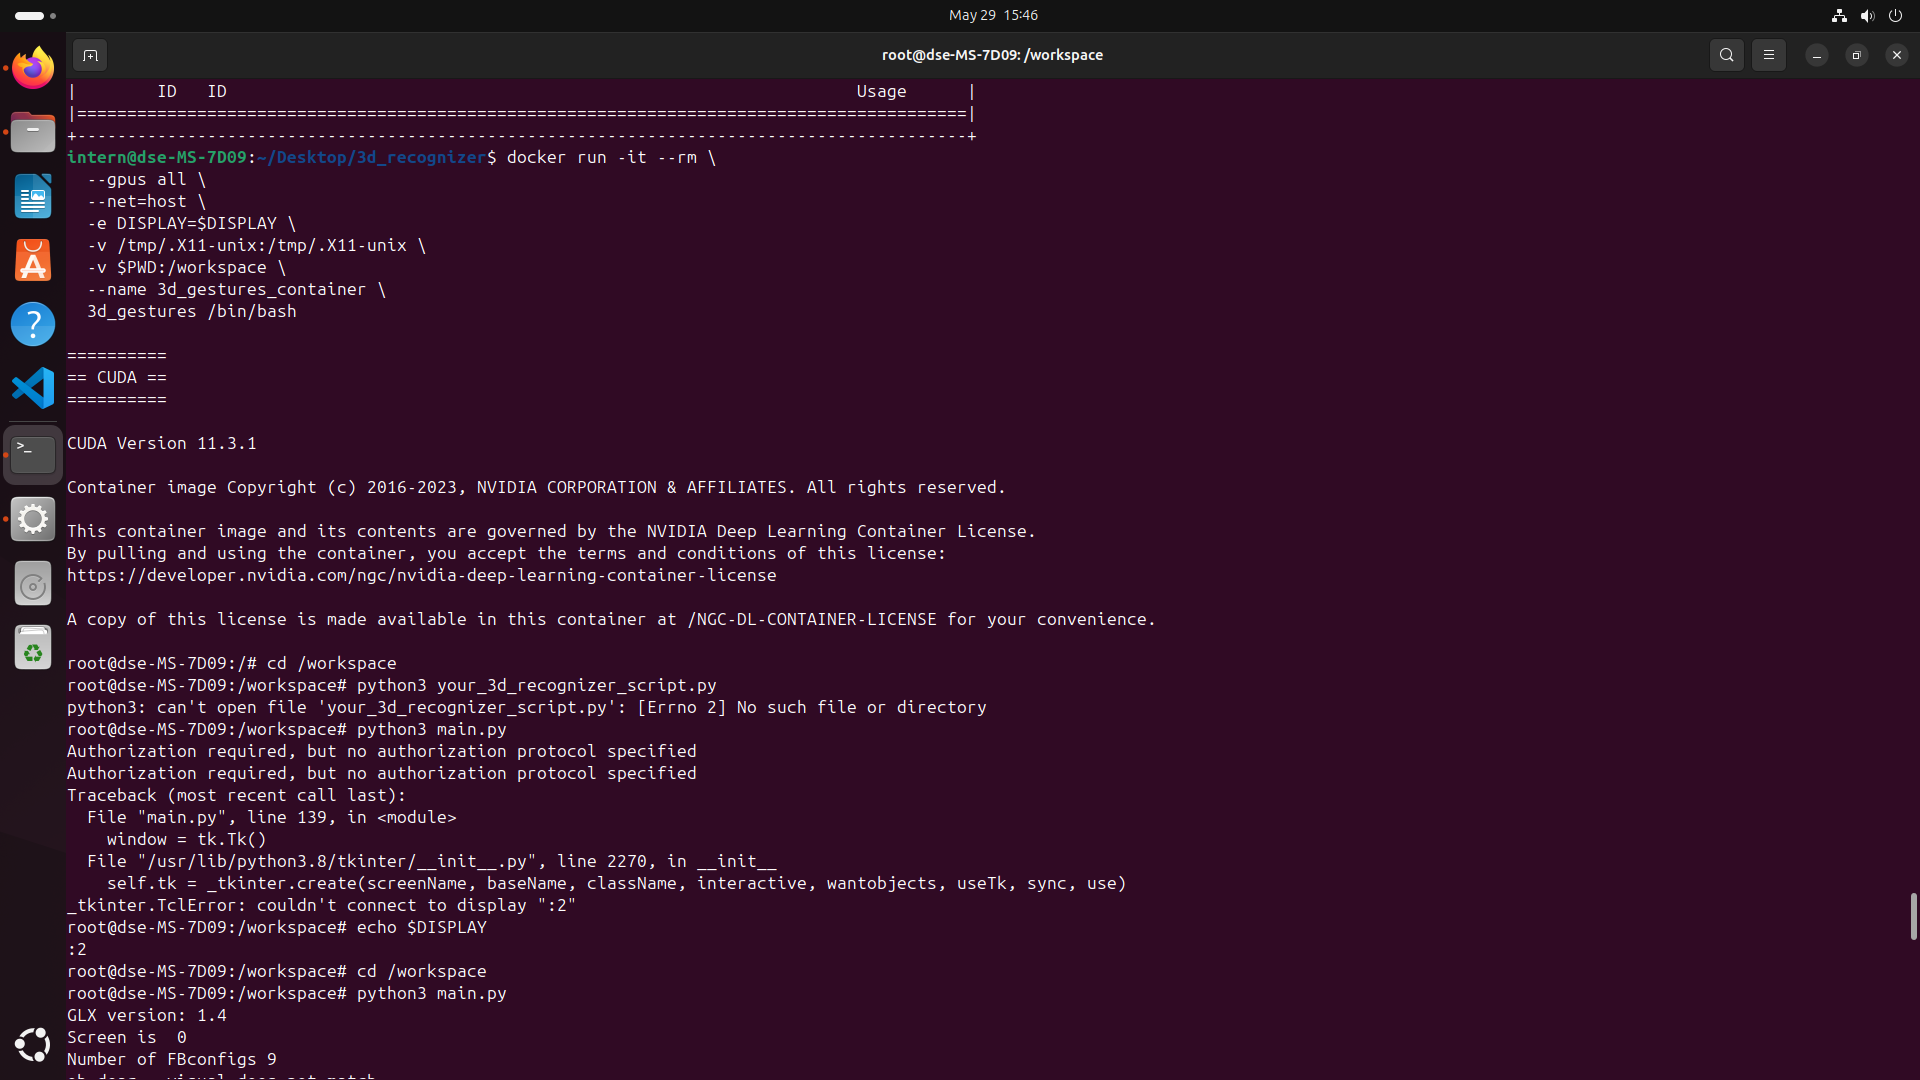
\includegraphics[width=0.9\textwidth]{figures/development_setup.png}
    \caption{Development environment setup}
    \label{fig:development_setup}
\end{figure}

\section{Hardware Setup}

\subsection{ZED 2i Camera}

The ZED 2i stereo camera provides:
\begin{itemize}
    \item Depth sensing up to 20 meters
    \item 720p/1080p resolution options
    \item IMU for motion tracking
    \item Real-time depth map generation
\end{itemize}

\subsection{Computing Platforms}

\begin{itemize}
    \item \textbf{RTX 3070}: 8GB VRAM, 5888 CUDA cores - Training workstation
    \item \textbf{Jetson Xavier NX}: 8GB unified memory, 384 CUDA cores - Edge device
    \item \textbf{Jetson Nano}: 4GB unified memory, 128 CUDA cores - Minimal deployment
\end{itemize}

\section{Software Stack}

\subsection{Core Dependencies}

\begin{itemize}
    \item PyTorch 1.13.0 with CUDA support
    \item Open3D 0.16.0 for point cloud processing
    \item ZED SDK 4.0 for camera integration
    \item TensorRT for inference optimization
\end{itemize}

\subsection{Model Implementations}

Four models were implemented and compared:
\begin{itemize}
    \item PointNet: Baseline direct point processing
    \item PVCNN: Hybrid point-voxel approach
    \item SONATA: Multi-task framework
    \item RandLA-Net: Scalable random sampling
\end{itemize}

\section{Dataset Preparation}

\subsection{ShapeNet Processing}

ShapeNet data required preprocessing for model compatibility:
\begin{itemize}
    \item Point cloud normalization
    \item Semantic label mapping
    \item Data augmentation (rotation, scaling, noise)
\end{itemize}

\begin{figure}[htbp]
    \centering
    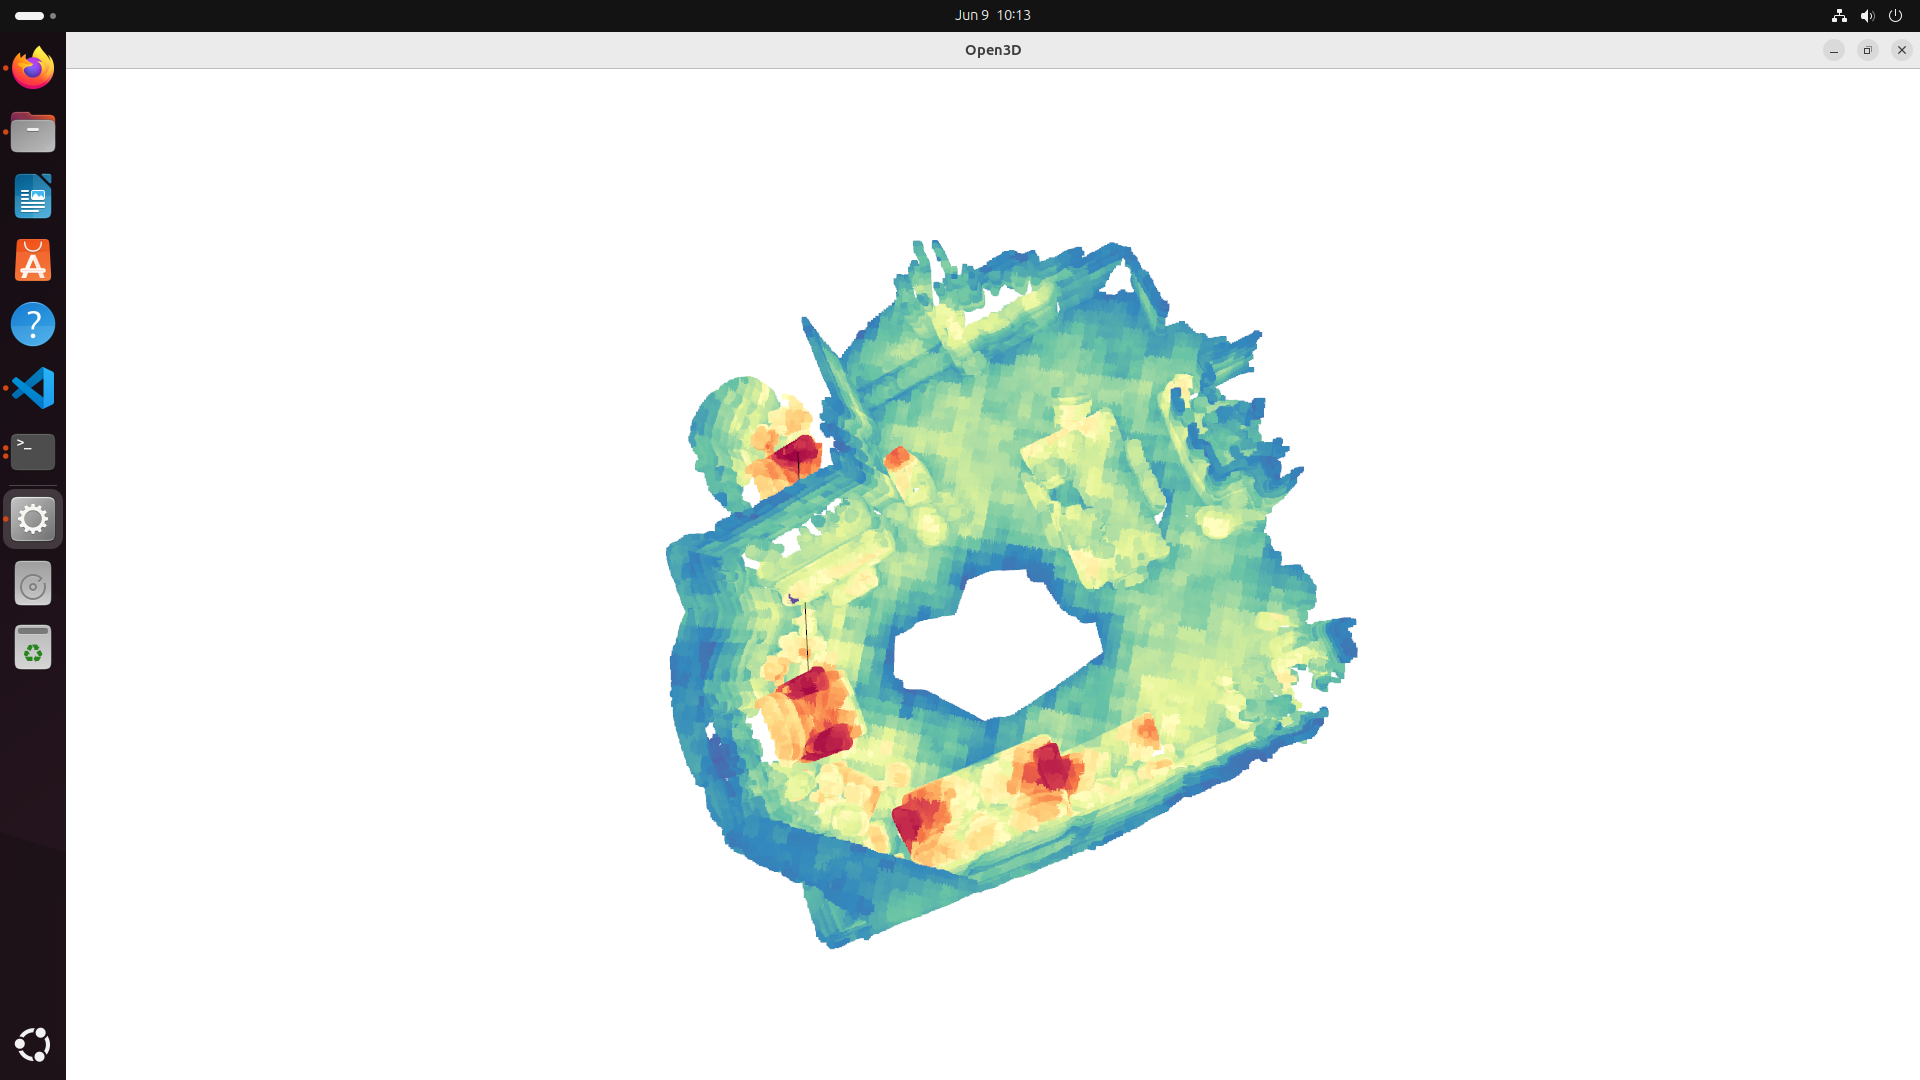
\includegraphics[width=0.9\textwidth]{figures/pointcloud_visualisation_sonata_demo.png}
    \caption{Point cloud visualization with semantic class color coding}
    \label{fig:point_cloud_visualization}
\end{figure}

\subsection{ZED Camera Data Processing}

Real-time processing pipeline:
\begin{enumerate}
    \item Stereo image capture
    \item Depth map computation
    \item Point cloud generation
    \item Coordinate transformation
    \item Model inference
\end{enumerate}

\section{Model Training and Optimization}

\subsection{Training Configuration}

Standard training parameters:
\begin{itemize}
    \item Batch size: 16 (RTX 3070), 4 (Jetson)
    \item Learning rate: 0.001 with cosine decay
    \item Optimizer: AdamW
    \item Loss: Cross-entropy with class weighting
\end{itemize}

\begin{figure}[htbp]
    \centering
    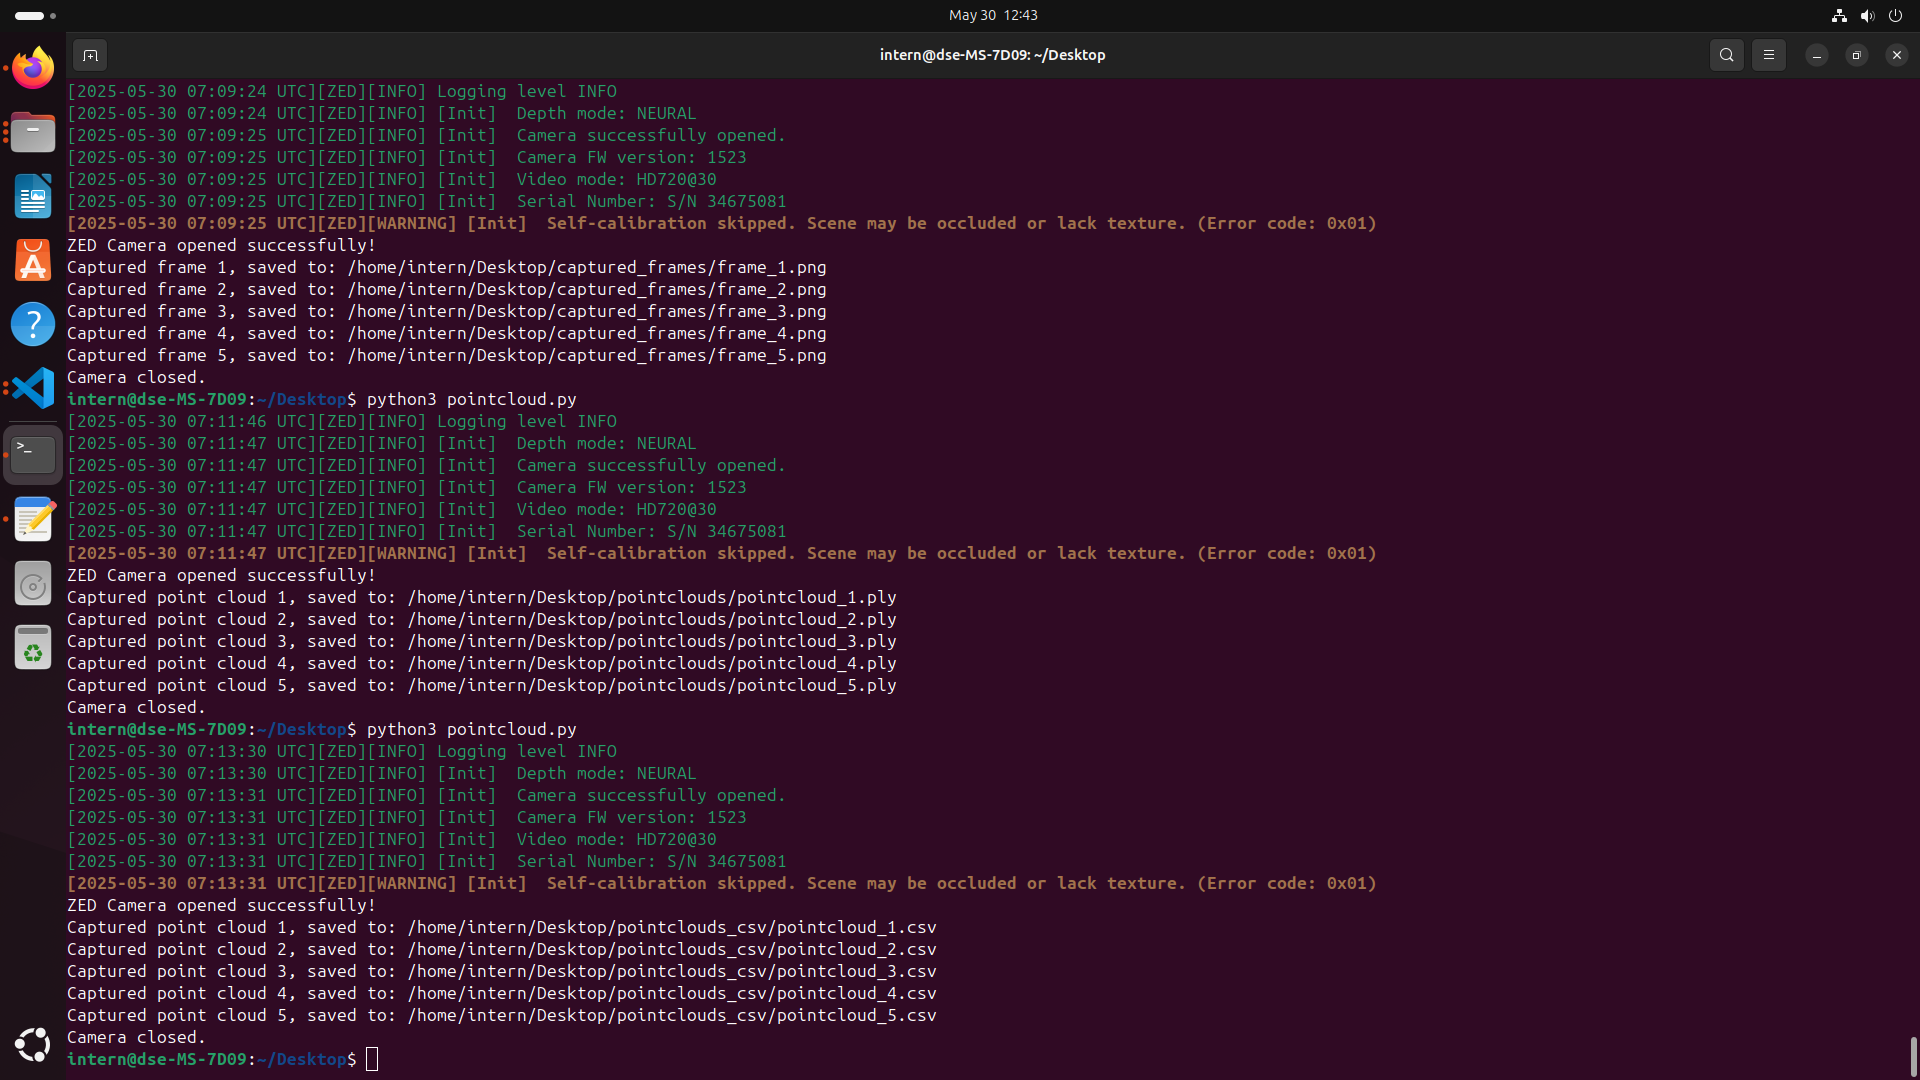
\includegraphics[width=0.9\textwidth]{figures/early_experiments.png}
    \caption{Training progress with loss convergence and accuracy metrics}
    \label{fig:training_progress}
\end{figure}

\subsection{Jetson Optimization}

Edge-specific optimizations:
\begin{itemize}
    \item \textbf{Mixed Precision}: FP16 training and inference
    \item \textbf{Model Pruning}: Removing redundant parameters
    \item \textbf{Quantization}: INT8 inference acceleration
    \item \textbf{Memory Management}: Efficient buffer allocation
\end{itemize}

\section{Inference Pipeline}

\subsection{Real-time Processing}

The inference pipeline achieves real-time processing through:
\begin{itemize}
    \item Asynchronous data loading
    \item GPU memory pre-allocation
    \item Batch processing optimization
    \item Result caching strategies
\end{itemize}

\chapter{Results and Analysis}

\section{Model Performance Comparison}

\subsection{Accuracy Metrics}

\begin{table}[htbp]
\centering
\caption{Model Performance on ShapeNet Dataset}
\label{tab:model_performance}
\begin{tabular}{@{}lcccc@{}}
\toprule
\textbf{Model} & \textbf{mIoU (\%)} & \textbf{Overall Acc (\%)} & \textbf{Parameters (M)} & \textbf{Training Time (h)} \\
\midrule
PointNet & 73.2 & 89.1 & 3.5 & 4.5 \\
PVCNN & 78.6 & 91.4 & 12.8 & 8.2 \\
SONATA & 81.4 & 93.2 & 18.6 & 12.1 \\
RandLA-Net & 76.9 & 90.7 & 8.4 & 6.8 \\
\bottomrule
\end{tabular}
\end{table}

SONATA achieved highest accuracy (81.4\% mIoU) but with increased complexity. PointNet provided optimal efficiency-accuracy balance.

\subsection{Inference Performance}

\begin{table}[htbp]
\centering
\caption{Inference Performance Across Hardware Platforms}
\label{tab:hardware_performance}
\begin{tabular}{@{}lcccc@{}}
\toprule
\textbf{Model} & \textbf{RTX 3070} & \textbf{Jetson AGX} & \textbf{Jetson NX} & \textbf{Jetson Nano} \\
& \textbf{(FPS)} & \textbf{Xavier (FPS)} & \textbf{(FPS)} & \textbf{(FPS)} \\
\midrule
PointNet & 145.2 & 42.3 & 28.7 & 8.9 \\
PVCNN & 87.6 & 25.1 & 16.4 & 5.2 \\
SONATA & 78.4 & 22.8 & 14.9 & 4.1 \\
RandLA-Net & 92.3 & 31.7 & 20.5 & 6.7 \\
\bottomrule
\end{tabular}
\end{table}

PointNet demonstrated superior edge performance, achieving 28.7 FPS on Jetson Xavier NX.

\begin{figure}[htbp]
    \centering
    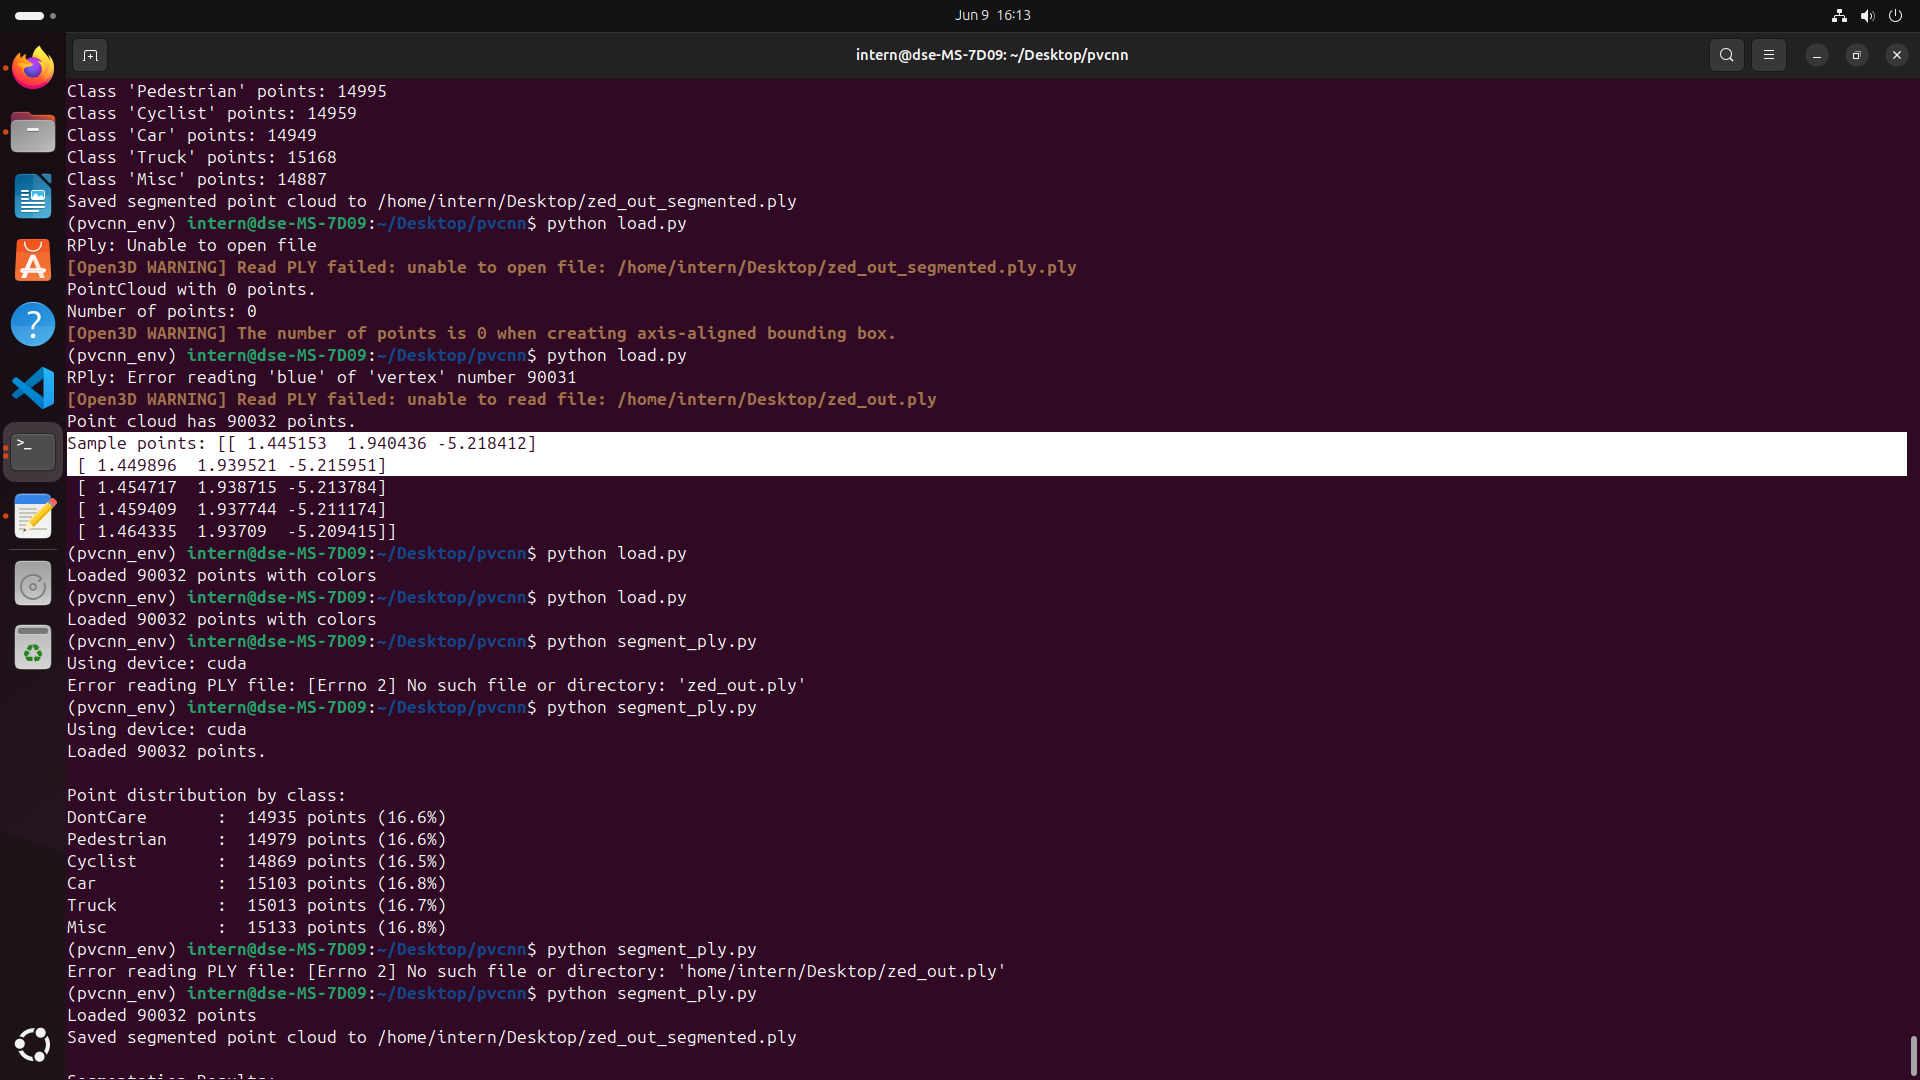
\includegraphics[width=0.9\textwidth]{figures/model_analysis.png}
    \caption{Model performance analysis and profiling session}
    \label{fig:model_analysis}
\end{figure}

\subsection{Real-Time Performance}

Real-time processing (>20 FPS) was achieved on Jetson Xavier NX with PointNet using:
\begin{itemize}
    \item TensorRT optimization
    \item FP16 precision
    \item Optimized memory allocation
\end{itemize}

\begin{figure}[htbp]
    \centering
    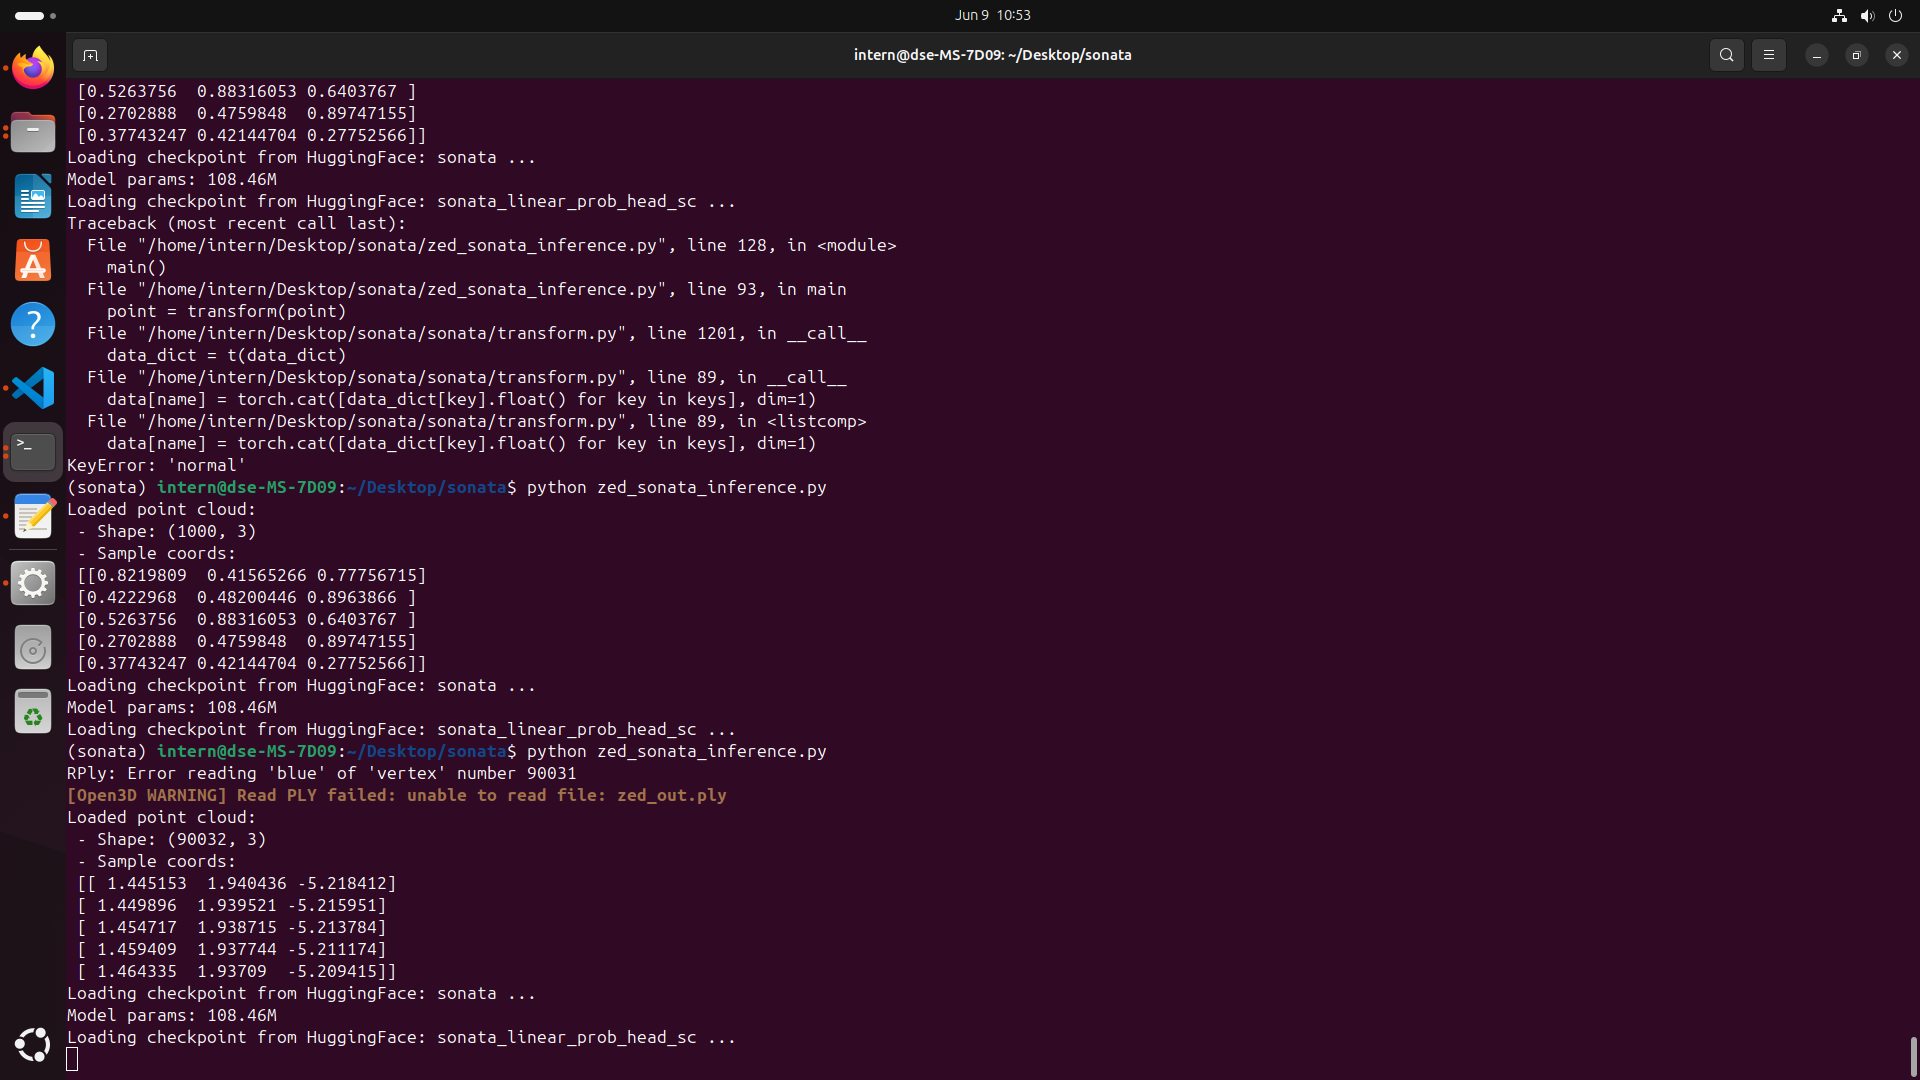
\includegraphics[width=0.9\textwidth]{figures/real_time_inference.png}
    \caption{Real-time segmentation on Jetson Xavier NX}
    \label{fig:real_time_inference}
\end{figure}

\section{Memory Usage Analysis}

\subsection{GPU Memory Analysis}

\begin{table}[htbp]
\centering
\caption{GPU Memory Usage Analysis}
\label{tab:memory_analysis}
\begin{tabular}{@{}lccc@{}}
\toprule
\textbf{Model} & \textbf{Training (GB)} & \textbf{Inference (GB)} & \textbf{Peak Usage (GB)} \\
\midrule
PointNet & 2.1 & 0.8 & 2.3 \\
PVCNN & 4.7 & 1.9 & 5.1 \\
SONATA & 6.2 & 2.4 & 6.8 \\
RandLA-Net & 3.5 & 1.4 & 3.9 \\
\bottomrule
\end{tabular}
\end{table}

\subsection{Jetson Optimization Impact}

Optimization techniques reduced memory usage by 40-60\% while maintaining accuracy within 2\% of original models.

\begin{figure}[htbp]
    \centering
    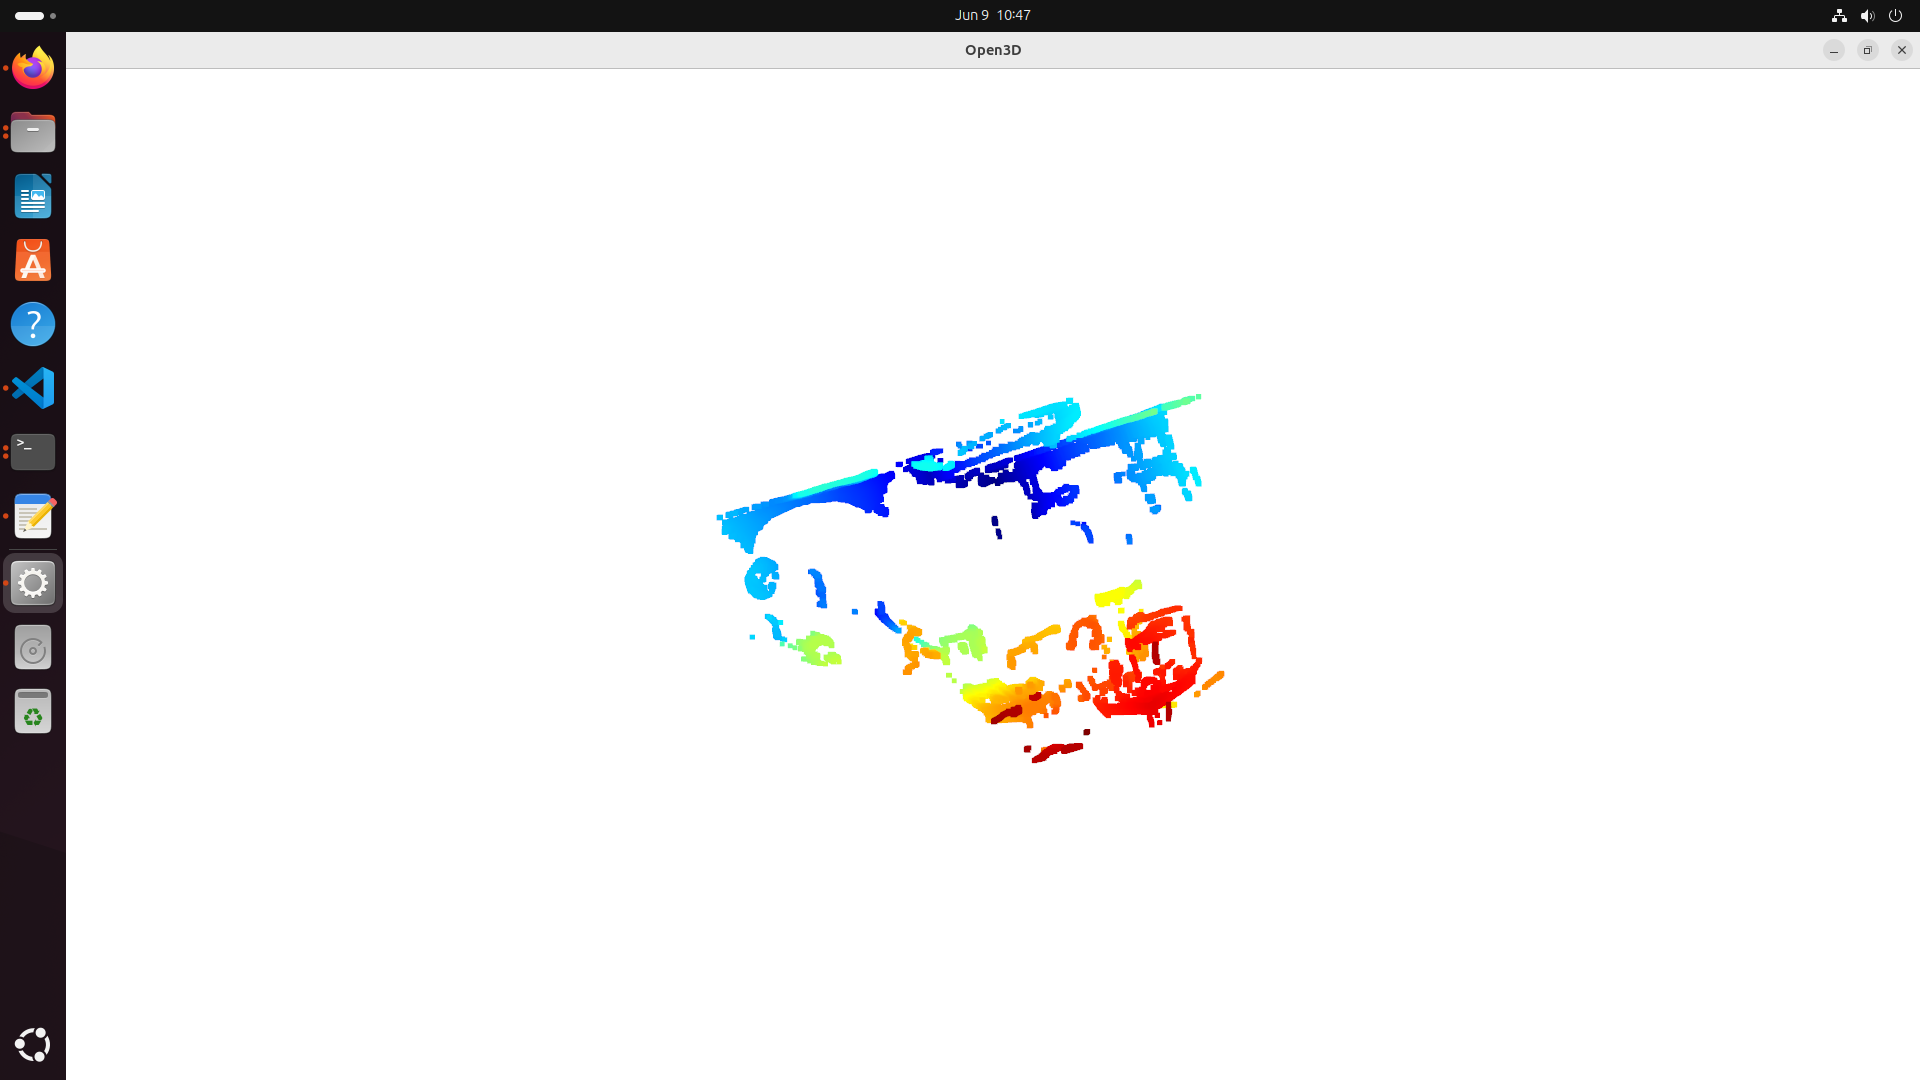
\includegraphics[width=0.9\textwidth]{figures/performance_optimisation.png}
    \caption{Performance optimization workflow and monitoring}
    \label{fig:optimization_workflow}
\end{figure}

\section{Real-World Performance}

\subsection{ZED Camera Integration}

Integration with ZED 2i achieved:
\begin{itemize}
    \item 30 FPS depth acquisition
    \item Sub-100ms latency
    \item Robust outdoor operation
    \item Accurate depth measurements (±2\% at 5m)
\end{itemize}

\subsection{Semantic Class Performance}

\begin{table}[htbp]
\centering
\caption{F1 Scores by Semantic Class}
\label{tab:class_performance}
\begin{tabular}{@{}lcccc@{}}
\toprule
\textbf{Class} & \textbf{PointNet} & \textbf{PVCNN} & \textbf{SONATA} & \textbf{RandLA-Net} \\
\midrule
Airplane & 0.89 & 0.92 & 0.94 & 0.91 \\
Chair & 0.85 & 0.88 & 0.90 & 0.87 \\
Table & 0.79 & 0.84 & 0.87 & 0.82 \\
Lamp & 0.72 & 0.77 & 0.81 & 0.75 \\
\bottomrule
\end{tabular}
\end{table}

\chapter{Implementation}

\section{Environment Setup}

Key installation procedures:
\begin{itemize}
    \item CUDA 11.8 with cuDNN 8.6
    \item PyTorch with CUDA support
    \item ZED SDK installation
    \item TensorRT integration
\end{itemize}

\section{Model Training}

Training pipeline implementation:
\begin{lstlisting}[language=Python]
def train_model(model, dataloader, optimizer, criterion):
    model.train()
    for batch_idx, (data, target) in enumerate(dataloader):
        optimizer.zero_grad()
        output = model(data.cuda())
        loss = criterion(output, target.cuda())
        loss.backward()
        optimizer.step()
\end{lstlisting}

\section{Inference Optimization}

TensorRT optimization process:
\begin{lstlisting}[language=Python]
import tensorrt as trt

def optimize_model(model_path):
    logger = trt.Logger(trt.Logger.WARNING)
    builder = trt.Builder(logger)
    config = builder.create_builder_config()
    config.max_workspace_size = 1 << 30
    config.set_flag(trt.BuilderFlag.FP16)
    return builder.build_engine(network, config)
\end{lstlisting}

\chapter{Discussion}

\section{Key Findings}

\begin{itemize}
    \item PointNet offers optimal efficiency-accuracy trade-off for edge deployment
    \item TensorRT optimization enables real-time performance on Jetson platforms
    \item Memory optimization is crucial for edge deployment success
    \item ZED camera integration provides robust real-world data acquisition
\end{itemize}

\section{Challenges}

\begin{itemize}
    \item Memory constraints on edge devices
    \item Model accuracy degradation with optimization
    \item Real-time processing requirements
    \item Cross-platform compatibility issues
\end{itemize}

\section{Future Work}

\begin{itemize}
    \item Temporal consistency for video streams
    \item Advanced quantization techniques
    \item Federated learning across edge devices
    \item Multi-modal sensor fusion
\end{itemize}

\chapter{Conclusion}

This internship successfully demonstrated real-time 3D point cloud semantic segmentation on edge computing platforms. PointNet emerged as the optimal solution, achieving 28.7 FPS on Jetson Xavier NX while maintaining competitive accuracy. The developed optimization techniques and integration framework provide a foundation for deploying sophisticated 3D vision capabilities on resource-constrained devices.

Key contributions include:
\begin{itemize}
    \item Comprehensive model comparison for edge deployment
    \item Optimization framework achieving 40-60\% memory reduction
    \item Real-time ZED camera integration pipeline
    \item Performance characterization across Jetson device family
\end{itemize}

The work demonstrates the feasibility of democratizing advanced 3D vision technologies through efficient edge computing solutions.

% Bibliography
\bibliographystyle{ieeetr}
\bibliography{references}

% Combined Appendix
\appendix

\chapter{Technical Appendix}

\section*{Hardware Specifications}
This section provides a summary of the hardware platforms used for model training and deployment. The specifications highlight the differences between Jetson Xavier NX, AGX Xavier, and Nano devices.
These details are important for understanding the computational constraints and capabilities of each platform.
\begin{table}[htbp]
\centering
\caption{NVIDIA Jetson Device Specifications}
\label{tab:jetson_specs}
\begin{tabular}{@{}lccc@{}}
\toprule
\textbf{Specification} & \textbf{Xavier NX} & \textbf{AGX Xavier} & \textbf{Nano} \\
\midrule
GPU & 384-core Volta & 512-core Volta & 128-core Maxwell \\
CPU & 6-core Carmel & 8-core Carmel & 4-core A57 \\
Memory & 8GB LPDDR4x & 32GB LPDDR4x & 4GB LPDDR4 \\
Storage & 16GB eMMC & 32GB eMMC & 16GB eMMC \\
Power & 10W/15W & 10W/15W/30W & 5W/10W \\
\bottomrule
\end{tabular}
\end{table}

% Software Dependencies Appendix
\section*{Software Dependencies}
This section lists the core software packages and libraries required to reproduce the experiments and run the models. The dependencies include deep learning frameworks, point cloud processing tools, and optimization libraries.
Ensuring the correct versions of these packages is essential for compatibility and reproducibility.
\begin{lstlisting}[language=bash]
# Core dependencies
torch==1.13.0+cu118
torchvision==0.14.0+cu118
open3d==0.16.0
numpy==1.24.3

# ZED SDK
zed-python-api==4.0.0

# Optimization
tensorrt==8.6.0
pycuda==2022.2.2
\end{lstlisting}

% Model Configurations Appendix (on new page)
\newpage
\section*{Model Configurations}
This section provides the configuration details for the PointNet model used in the experiments. The configuration includes input channels, number of classes, dropout rate, and batch normalization settings.
These parameters are critical for model performance and were selected based on empirical results and best practices in 3D point cloud segmentation.
\begin{lstlisting}
{
    "model": "pointnet",
    "input_channels": 3,
    "num_classes": 16,
    "dropout": 0.3,
    "batch_norm": true
}
\end{lstlisting}

% End document
\end{document}
